\section{results}\label{sec:results}
\subsection{Generation results}\label{subsec:generation-results}
The results were made by measuring the generation time for a \gls{void} description for different database sizes. The database started at 1 million triples and was incremented by 10.000 triples up to 10.000.000. A \gls{void} description was generated for each increment for the database, and the time it took to generate it was measured in ms. This was done ten times to ensure the results would be reliable. From this, a graph could be made, and a linear regression could be made to show the trend of the generation time. This help to show how much the time to generate a \gls{void} description increases as the database size increases.

A graph of the standard deviation of the results can be seen in \autoref{fig:generate-dbsize-all}, which shows the size of the database along the x-axis and the generation time in ms on the y-axis. Each point in the graph has a span, the standard deviation of the results. From the graph, it is clear to see that there is a trend that the data follows. As the database size increases, so does the time it takes to generate a \gls{void} description; the time increases linearly with the database size.

\begin{figure}[htb!]
    \centering
    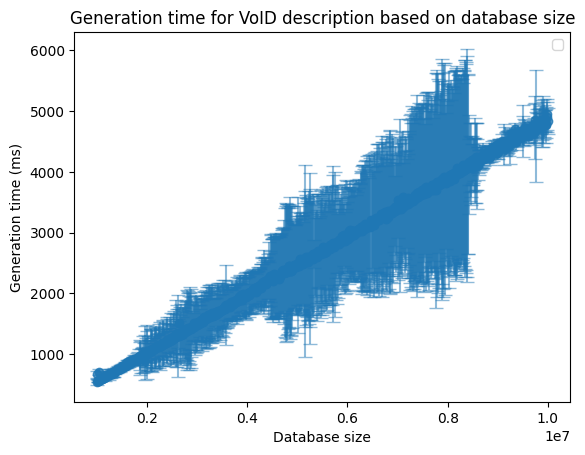
\includegraphics[width=0.8\columnwidth]{figures/generation-results-graph.png}
    \caption{2D graph showing the standard deriviation impact of database size on the time it takes to generate a VoID description. Containing all the data.}
    \label{fig:generate-dbsize-all}
\end{figure}

Though there is a strange trend when the database reaches the size above 8.000.000 triples, the standard deviation of the results suddenly decreases. To better understand why this happens, we can show a graph over all ten runs and see if anything could indicate why the sudden decrease happens. In \autoref{fig:generate-dbsize-10-runs-all}, we can see the results of all ten runs.

\begin{figure}[htb!]
    \centering
    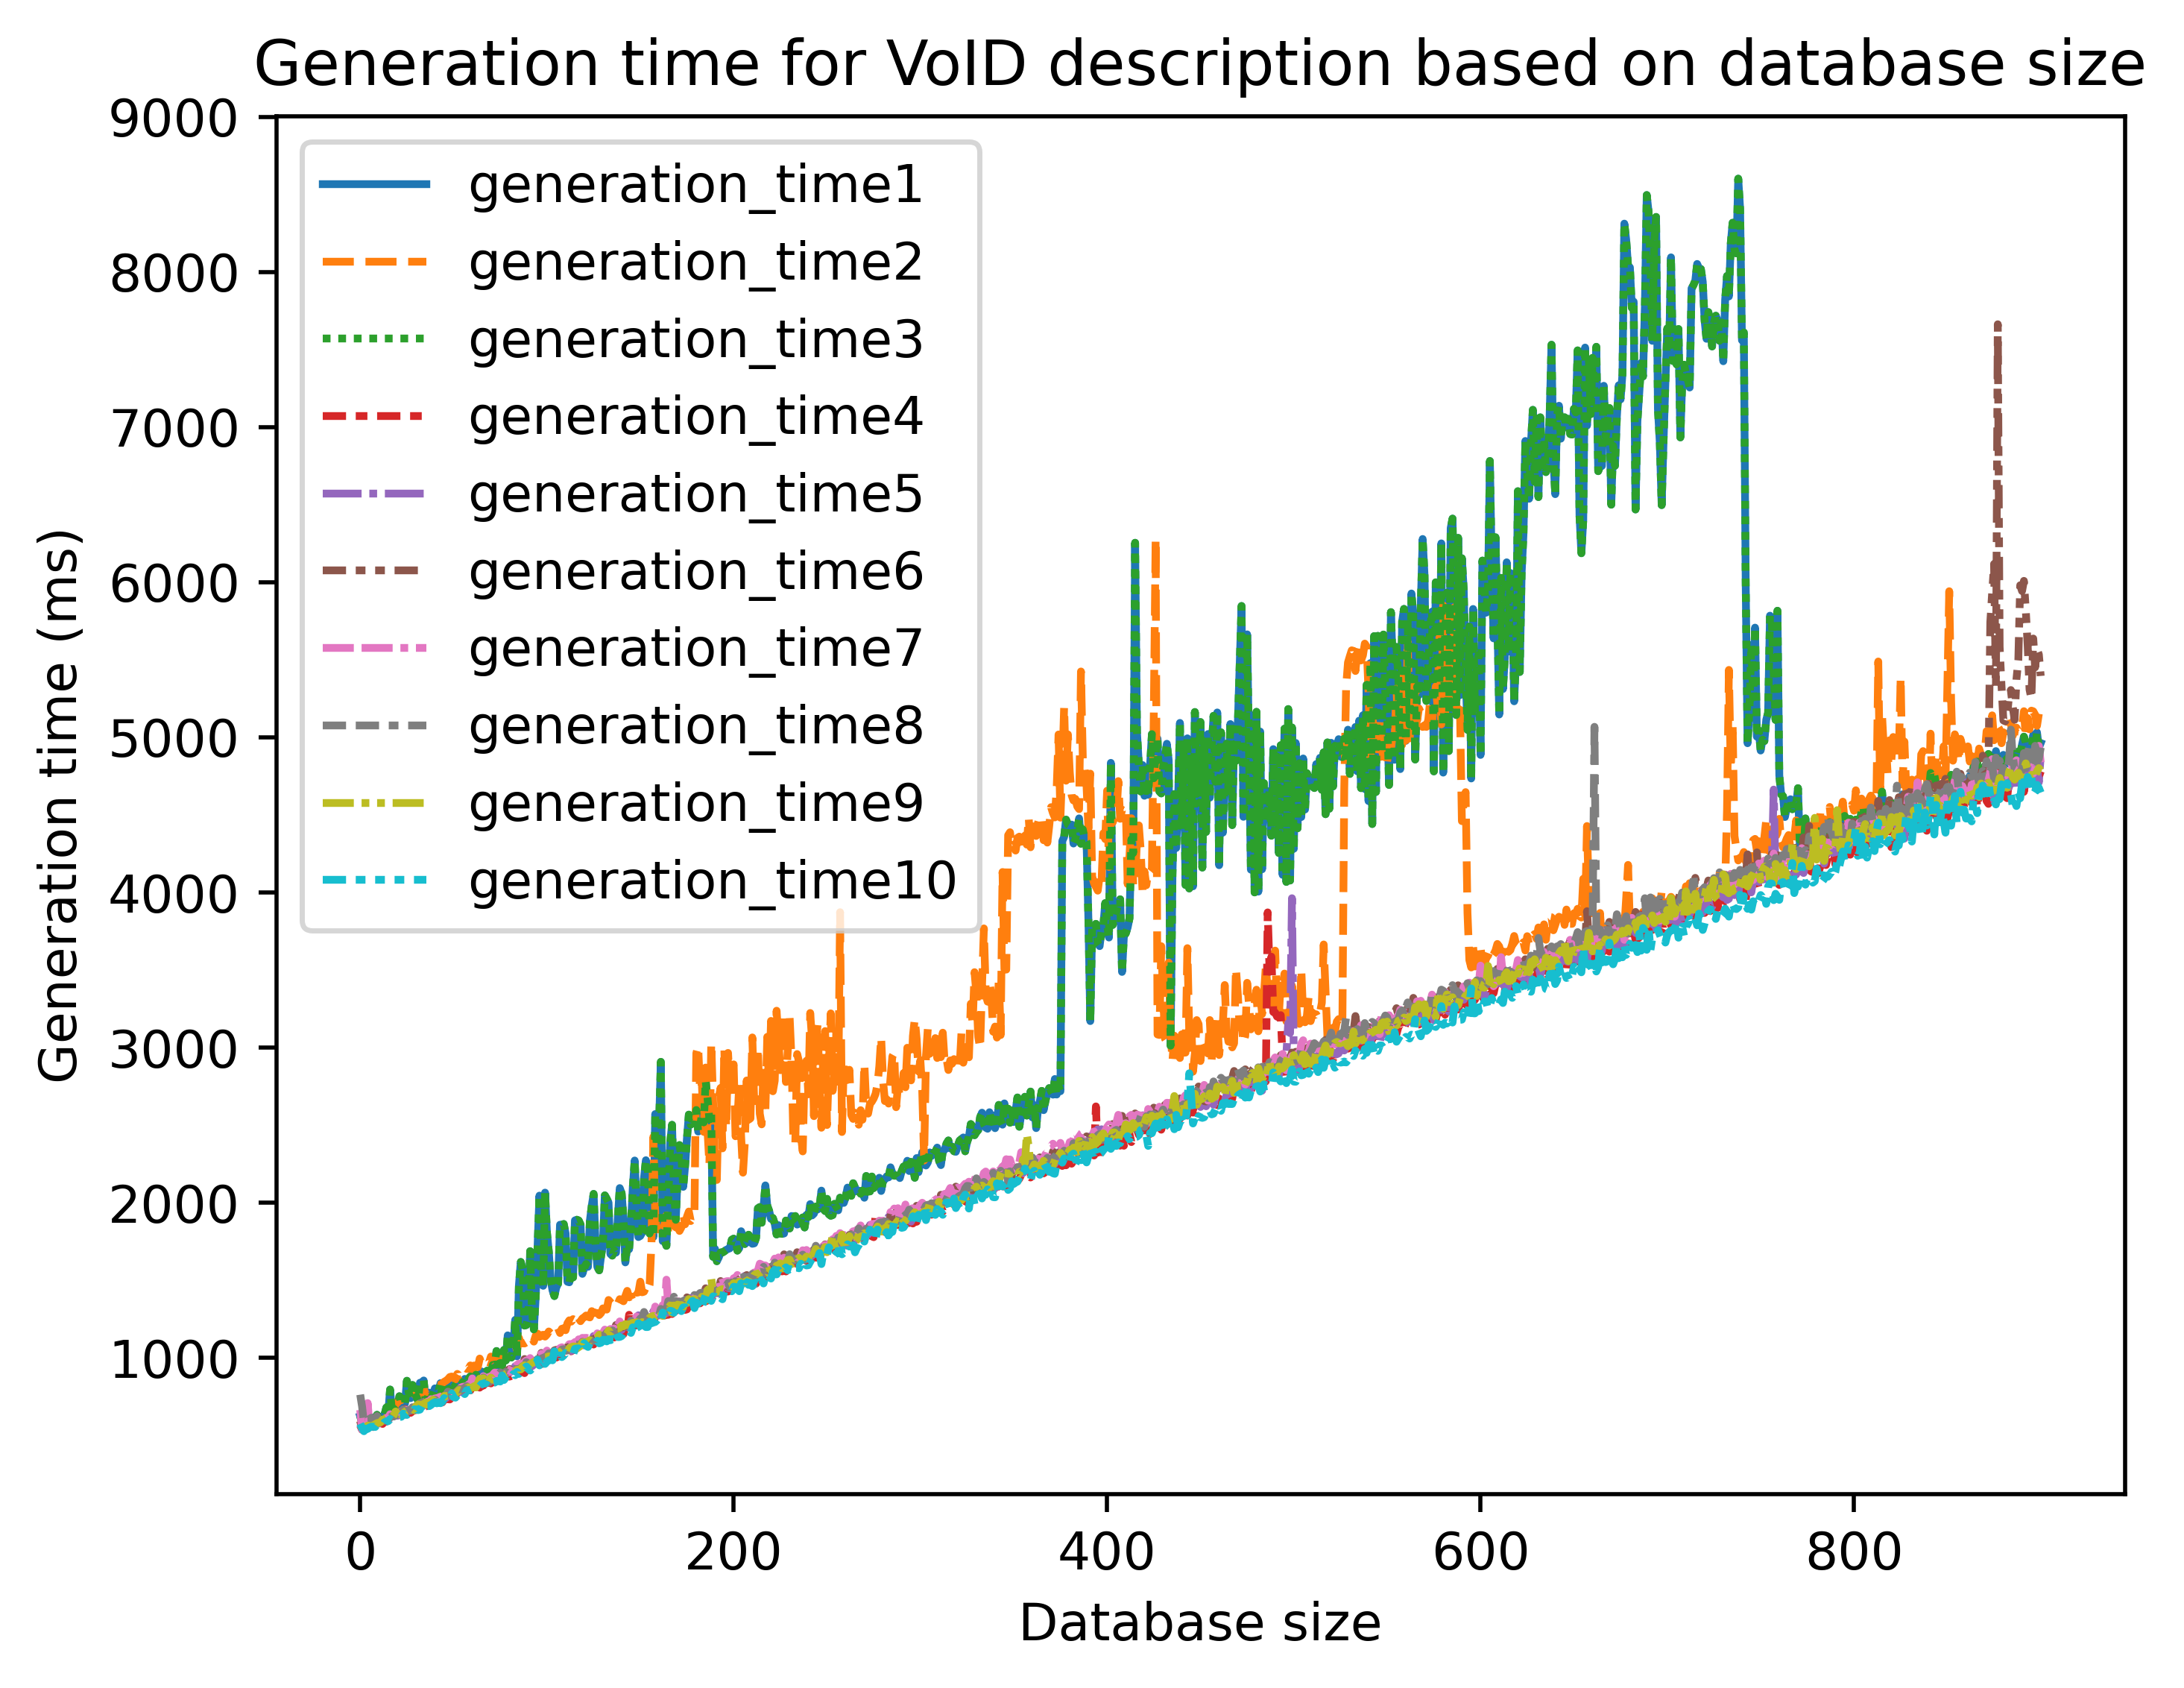
\includegraphics[width=0.8\columnwidth]{figures/generation-results-graph-all.png}
    \caption{2D graph showing each runs impact of database size on the time it takes to generate a VoID description. Containing all the data.}
    \label{fig:generate-dbsize-10-runs-all}
\end{figure}

Certain outliers deviate significantly from others. This is most likely because the computer running the measurements was in use during the first few runs. This has likely affected the results and caused the outliers. This can be even more seen when sorting these outliers out in \autoref{fig:generate-dbsize-10-runs-good}. In this graph, all the results are much more similar, showing that, when generating the results, it was susceptible to any other activity happening on the machine, thereby creating outliers. So by generating a new graph with the outliers removed, we can see that the standard deviation of the results is much more stable and still follows the same trend as before.

\begin{figure}[htb!]
    \centering
    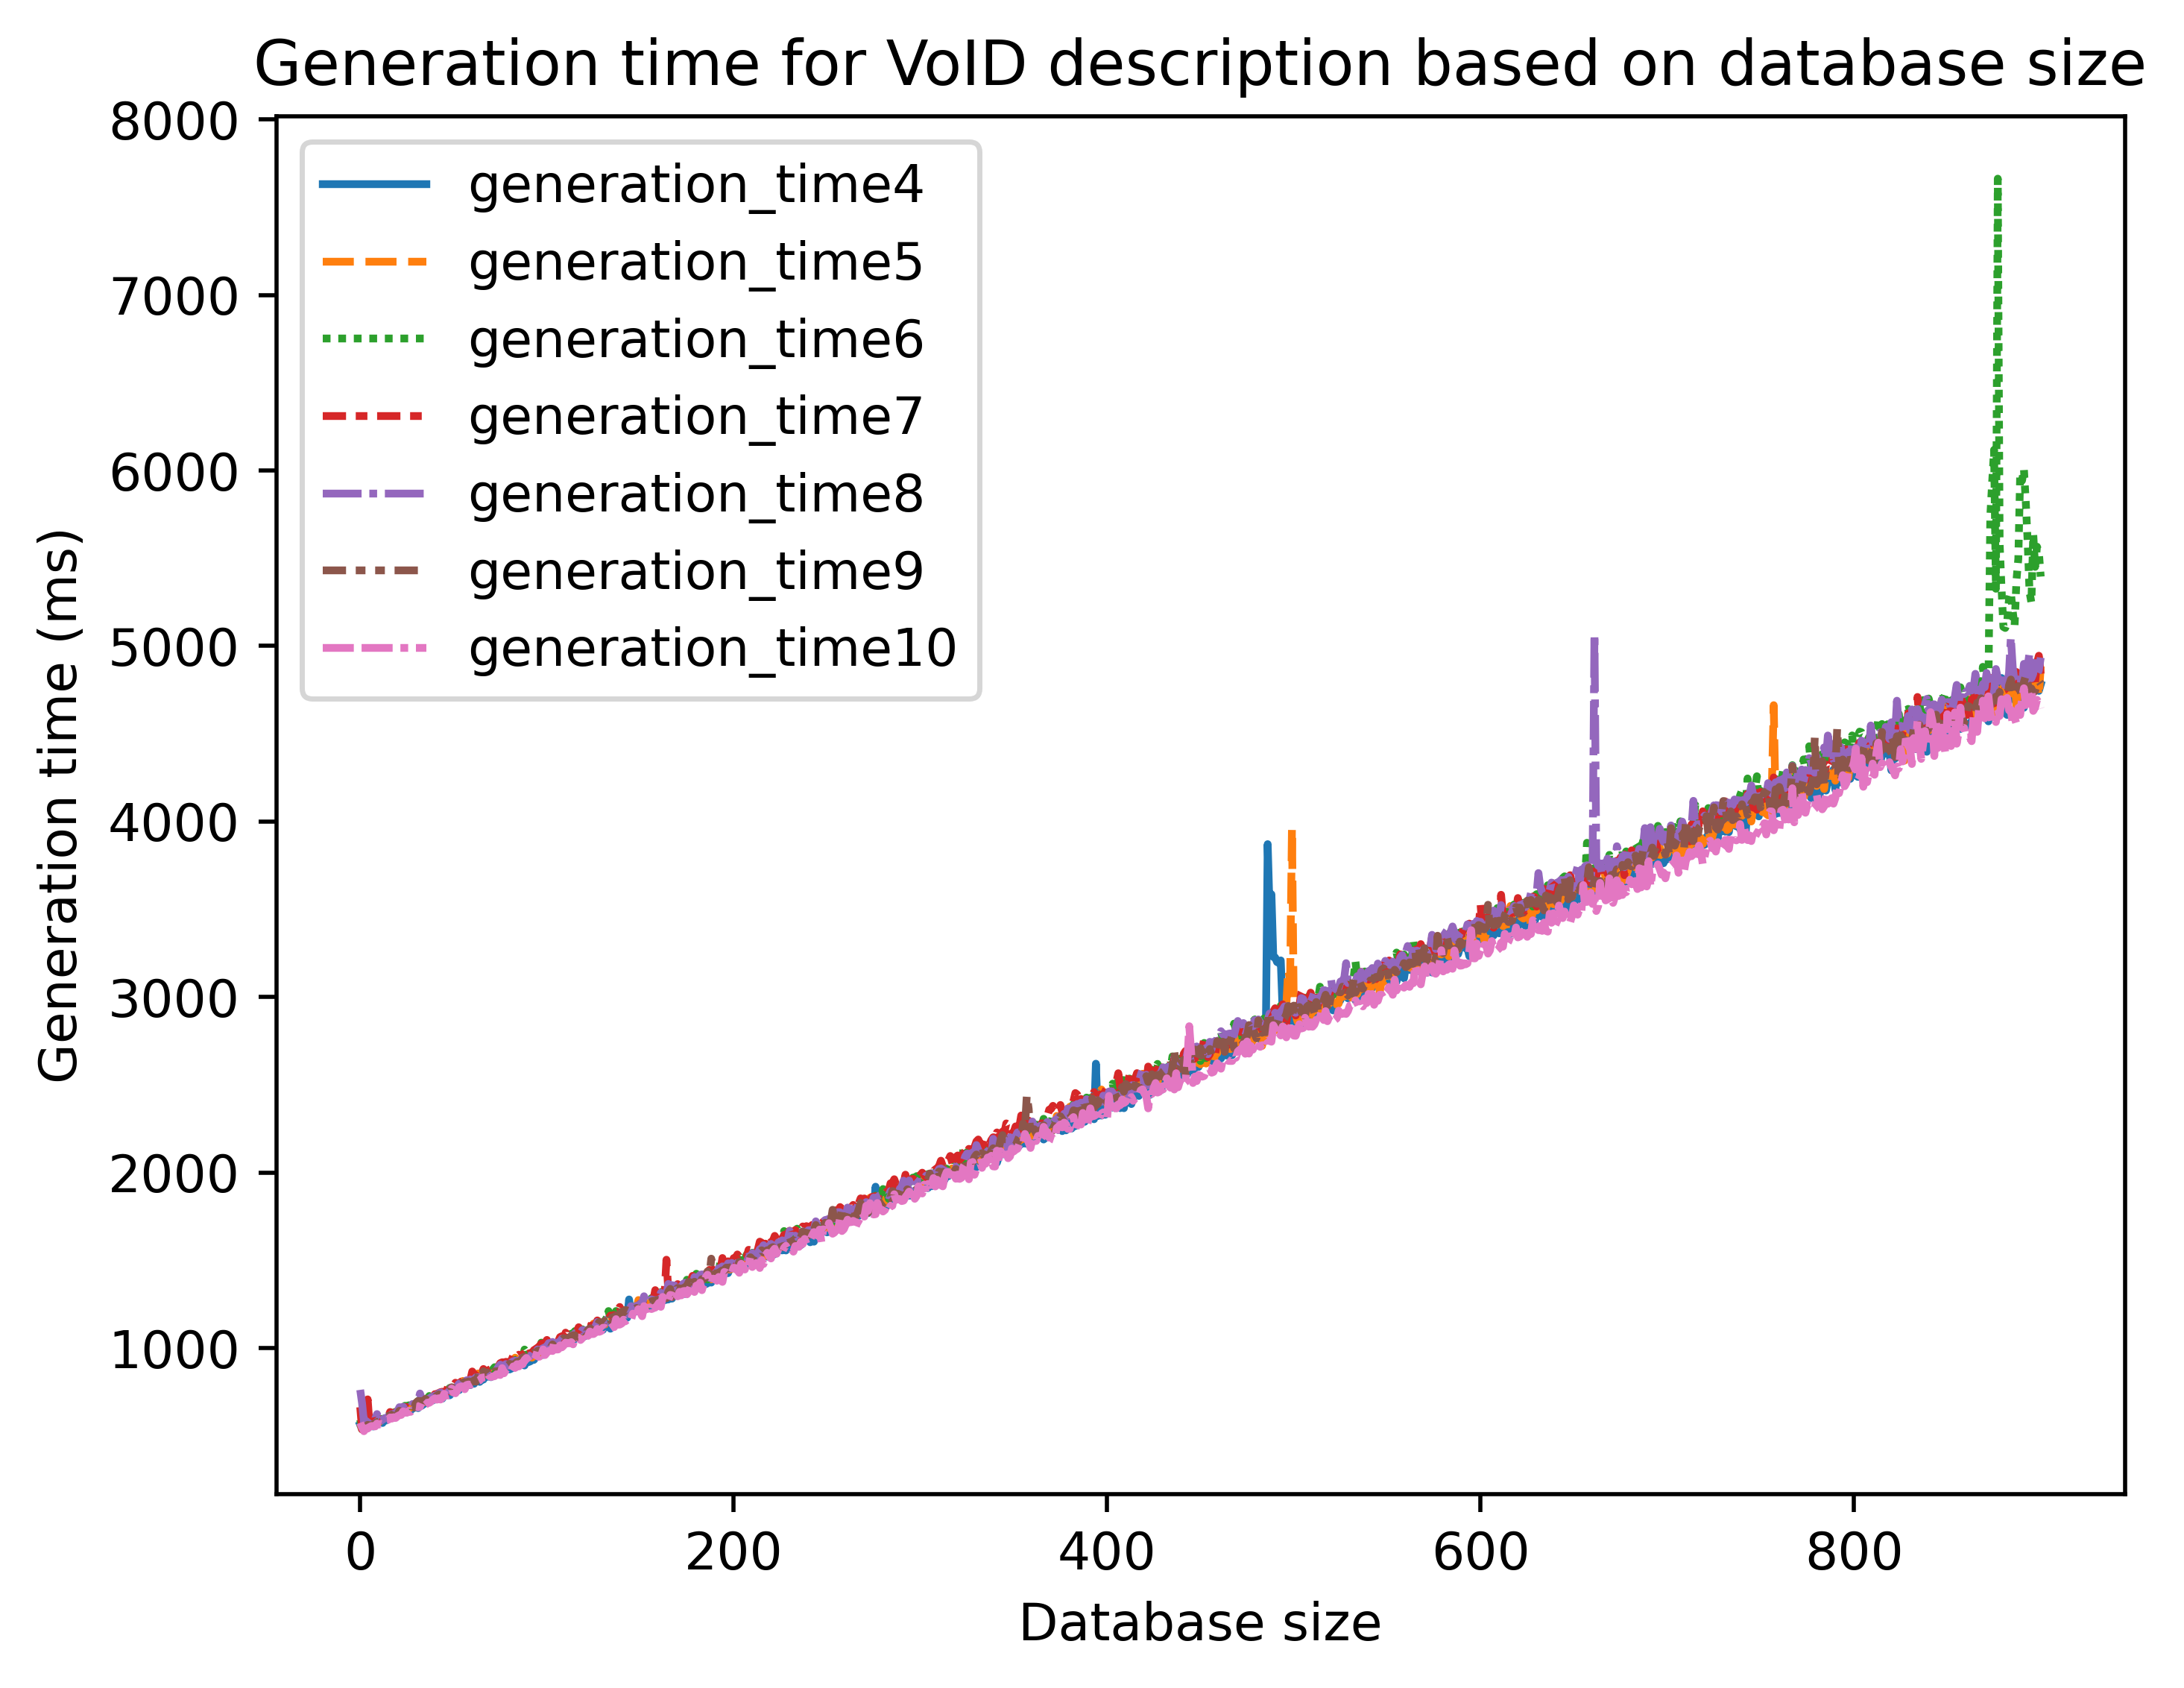
\includegraphics[width=0.8\columnwidth]{figures/generation-results-graph-all-good.png}
    \caption{2D graph showing each runs impact of database size on the time it takes to generate a VoID description. Containing only the good data.}
    \label{fig:generate-dbsize-10-runs-good}
\end{figure}

From this, we can gather that the time it takes to generate a \gls{void} description for a database linearly increases as the database size increases. This is expected as the more triples the database has, the more triples the script has to process and the longer it will take to generate the \gls{void} description.


\subsection{Update results}\label{subsec:update-results}
The results for updating the \gls{void} description contained three parameters: time, query size, and database size. The query size was measured when updating the \gls{void} description but not when generating it because query size did not affect generation, as the generation is purely based on what is in the database.

The results were made by measuring the time it took to update the \gls{void} description for database and query sizes. As in \autoref{subsec:generation-results}, the database started at 1 million triples and incremented by 10.000 triples up to 10.000.000. The query size starts at one triple and increases by 1.000 until reaching 8.001, whereafter the database increments by 10.000, and the query size starts at one again. For each change in the query size, a measurement is made for how long it takes to update the \gls{void} description.

Why the query size only ended at 8.001 and not by the 10.000 that was later inserted into the database because, looking at the data, the time it took to update the \gls{void} description grew linearly with the query size. Therefore, it was not necessary to test for query sizes above 8.001, as the time it took to update the \gls{void} description could be calculated by making a linear regression of the data and saving time on the measurements.

\task{Consider making an experiment that tests for updating new vs. updating existing data.}

The generation results were measured in increments of 10.000, where the VOID description was generated and the generation time was measured.

The update results were measured nine times for every 10.000 increments of the database size with different query sizes. The query size for each iteration started at one and was incremented by 1000 up to 8001. This means the update results have nine times more data than the generation results.

However, it is essential to note that the queries was never inserted into the database, because the queries were only used to update the \gls{void} description and not the database itself. Therefore it did not directly impact the database size and was not incremented by 1.000 for each query size increment.

As with \autoref{subsec:generation-results}, the first three runs was impacted by the computer used during the measurements. This can be seen in \autoref{fig:update-querysize-all}, where some outliers deviate significantly from the rest of the data. Because of the outliers, we are mainly interested in the data generated without the computer being used, as this data is more reliable, as seen in \autoref{fig:update-querysize-good}.

\begin{figure}[htb!]
    \centering
    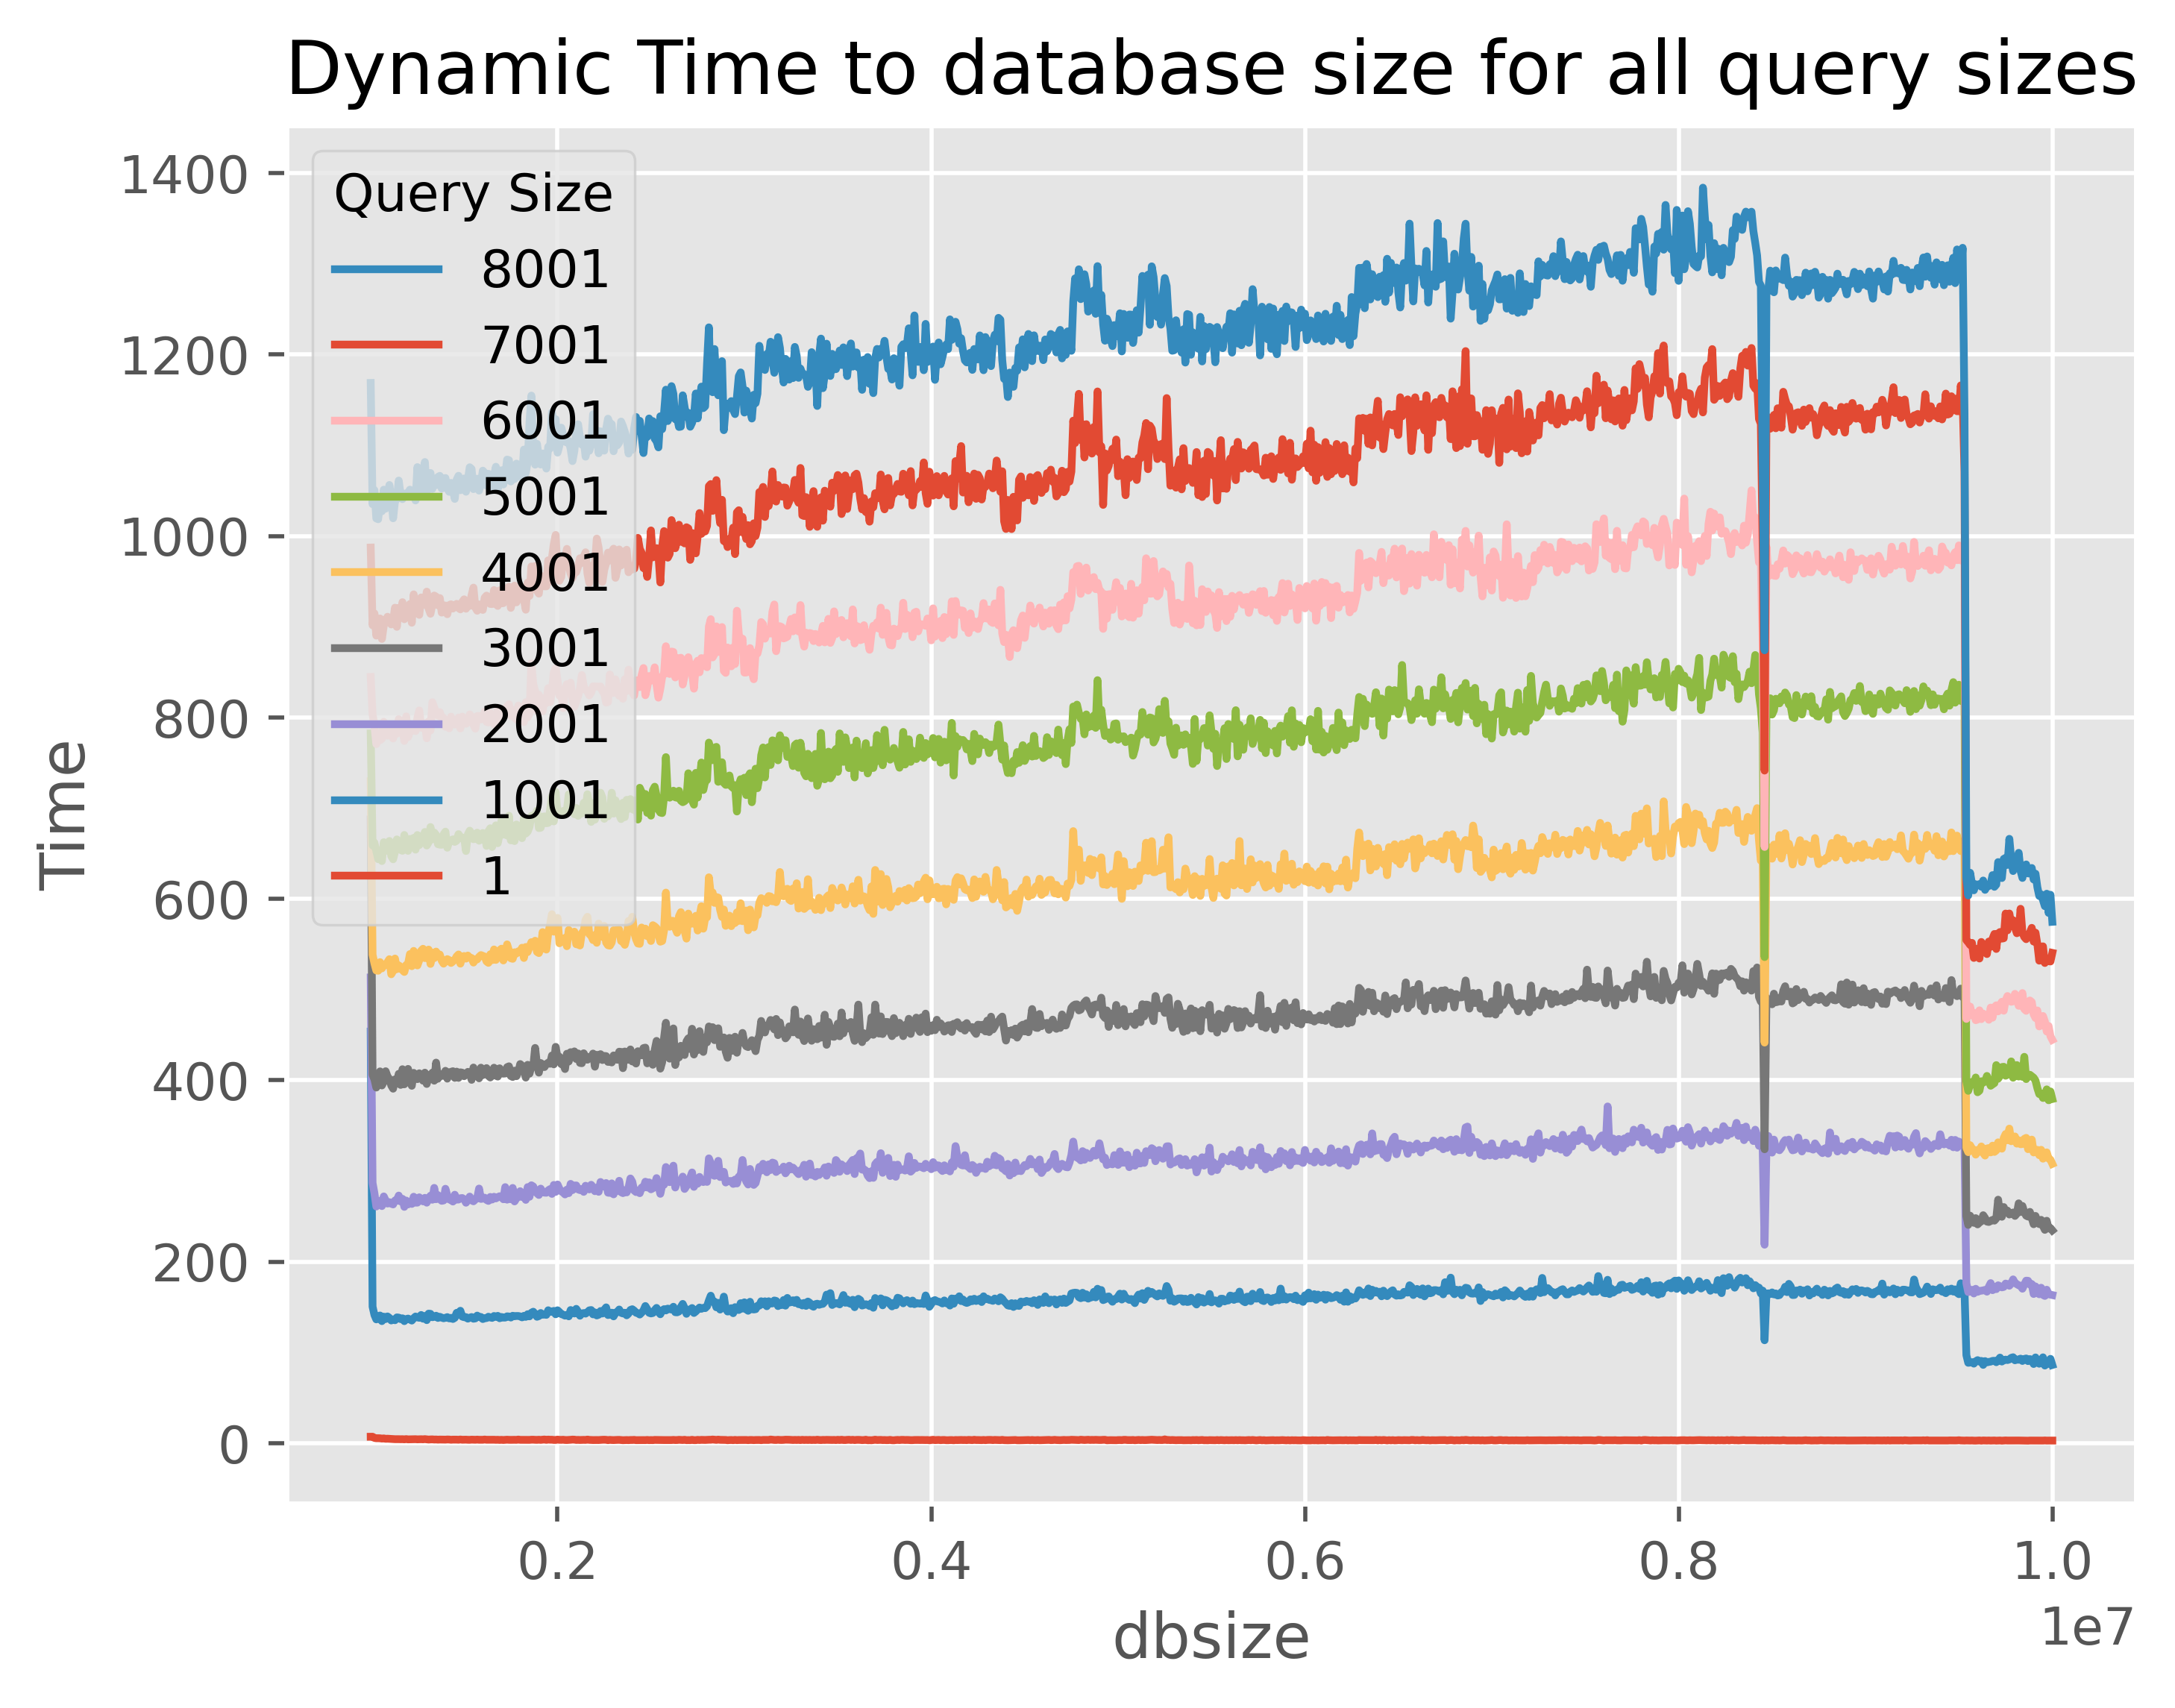
\includegraphics[width=0.8\columnwidth]{figures/dynamic-time-query-size-all.png}
    \caption{2D graph showing the impact of query size and database size on the time it takes to update a VoID description, containing all the data.}
    \label{fig:update-querysize-all}
\end{figure}

\begin{figure}[htb!]
    \centering
    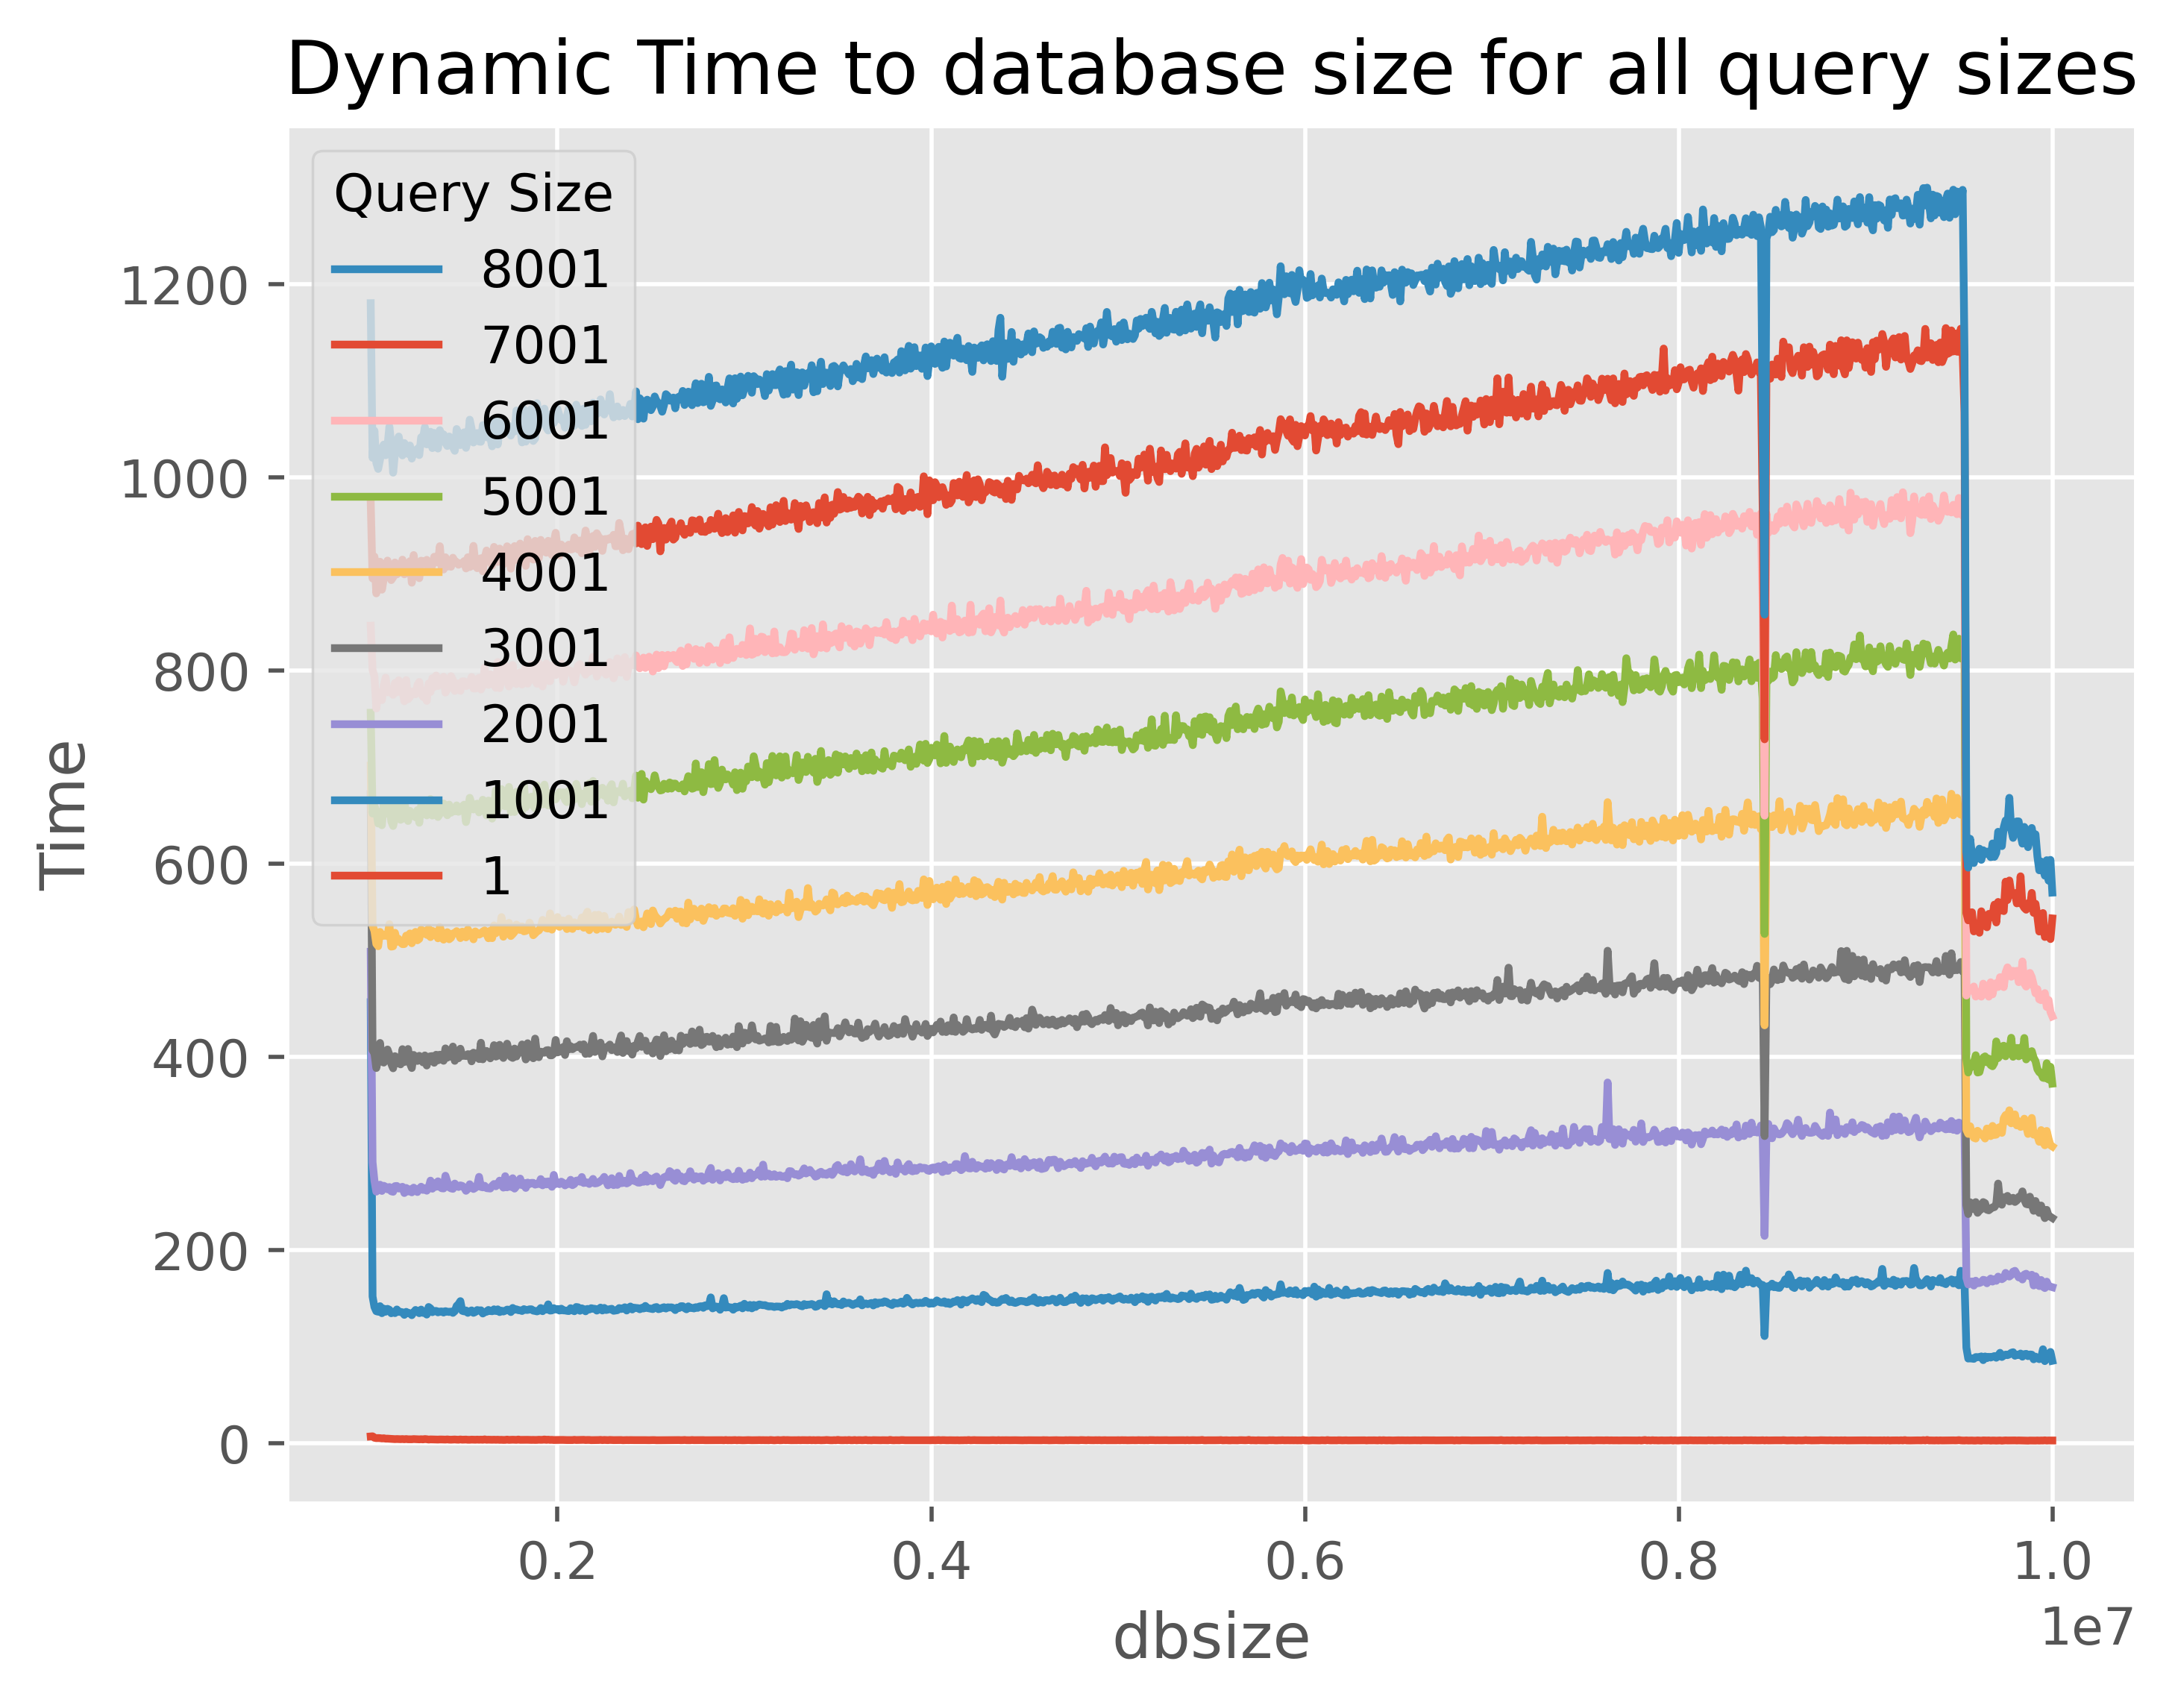
\includegraphics[width=0.8\columnwidth]{figures/dynamic-time-query-size-good.png}
    \caption{2D graph showing the impact of query size and database size on the time it takes to update a VoID description, containing only the good data.}
    \label{fig:update-querysize-good}
\end{figure}


The 2D-graph in \autoref{fig:update-querysize-good} shows the impact of query size and database size on the time it takes to update a \gls{void} description. From this graph, it is clear to see that there is a trend that the data follows.

The query size significantly impacts the time it takes to update the \gls{void} description, and the database size bearly impacts the time it takes to update the \gls{void} description. This is because as the amount of new data inserted into the database increases, so does the time to update the \gls{void} description because the script has to process more data. However, the query size impacts the time it takes to update the \gls{void} description much more, as the more triples the query contains, the more triples the script has to process and the longer it will take to update the \gls{void} description.

This is to be expected, as the more data inserted, the more data the script has to process and the longer it will take to update the \gls{void} description. However, all the data inserted is new, meaning it is currently unknown if updating existing data will significantly impact the time it takes to update the \gls{void} description.

This could be tested in the future, but it will likely not significantly impact the time it takes to update the \gls{void} description. This is because the script does not have to process the data that is already in the database, and therefore it will not impact the time it takes to update the \gls{void} description. However, it is not known for sure if this is the case, and it could be tested in the future.

A 2D graph was made to display the impact of database size and query size more clearly. In \autoref{fig:update-querysize-good}, we can see that the database size has a minor effect on the time to update, but the query size is the main factor in the time it takes to update the \gls{void} description.

There is an unexpected trend in the graph, where the time it takes to update the \gls{void} description suddenly decreases when the database is almost 10.000.000 triples. The decrease in time to update the VOID description did not appear to be directly related to the number of triples inserted. However, upon examining the inserted data, it was observed that its size was significantly smaller than the previous data.

This suggests that the structure of the data plays a significant role in the time required for updating the VOID description. However, it remains unclear which specific aspects of the data are primarily responsible for this effect. Factors such as the number of characters, data type, or other variables could contribute to the decrease in update time. Investigating how the data's structure influences the time needed to update the VOID description would be an intriguing area for future research.

From these findings, we can gather that the time it takes to update a \gls{void} description is heavily impacted by the size of the query (the number of characters in the query) that is being inserted and not so much the size of the database.


\subsection{Update and generation comparison}\label{subsec:update-generation-comparison}
\autoref{fig:comparison-generation-vs-update}, shows a 2D graph of the impact of database size on the time it takes to generate a \gls{void} description and the time it takes to update a \gls{void} description. Since generating a \gls{void} description is greatly affected by the size of the database, the time it takes to generate a \gls{void} description increases significantly faster than the time it takes to update a \gls{void} description.

In comparison, the database size barely affects the nine update measurements for each query size. From this, it can be gathered that the larger the database is, the more it makes sense to update the \gls{void} description instead of generating it from scratch, but with a smaller database, it makes more sense to generate the \gls{void} description from scratch.

\begin{figure*}[t]
    \centering
    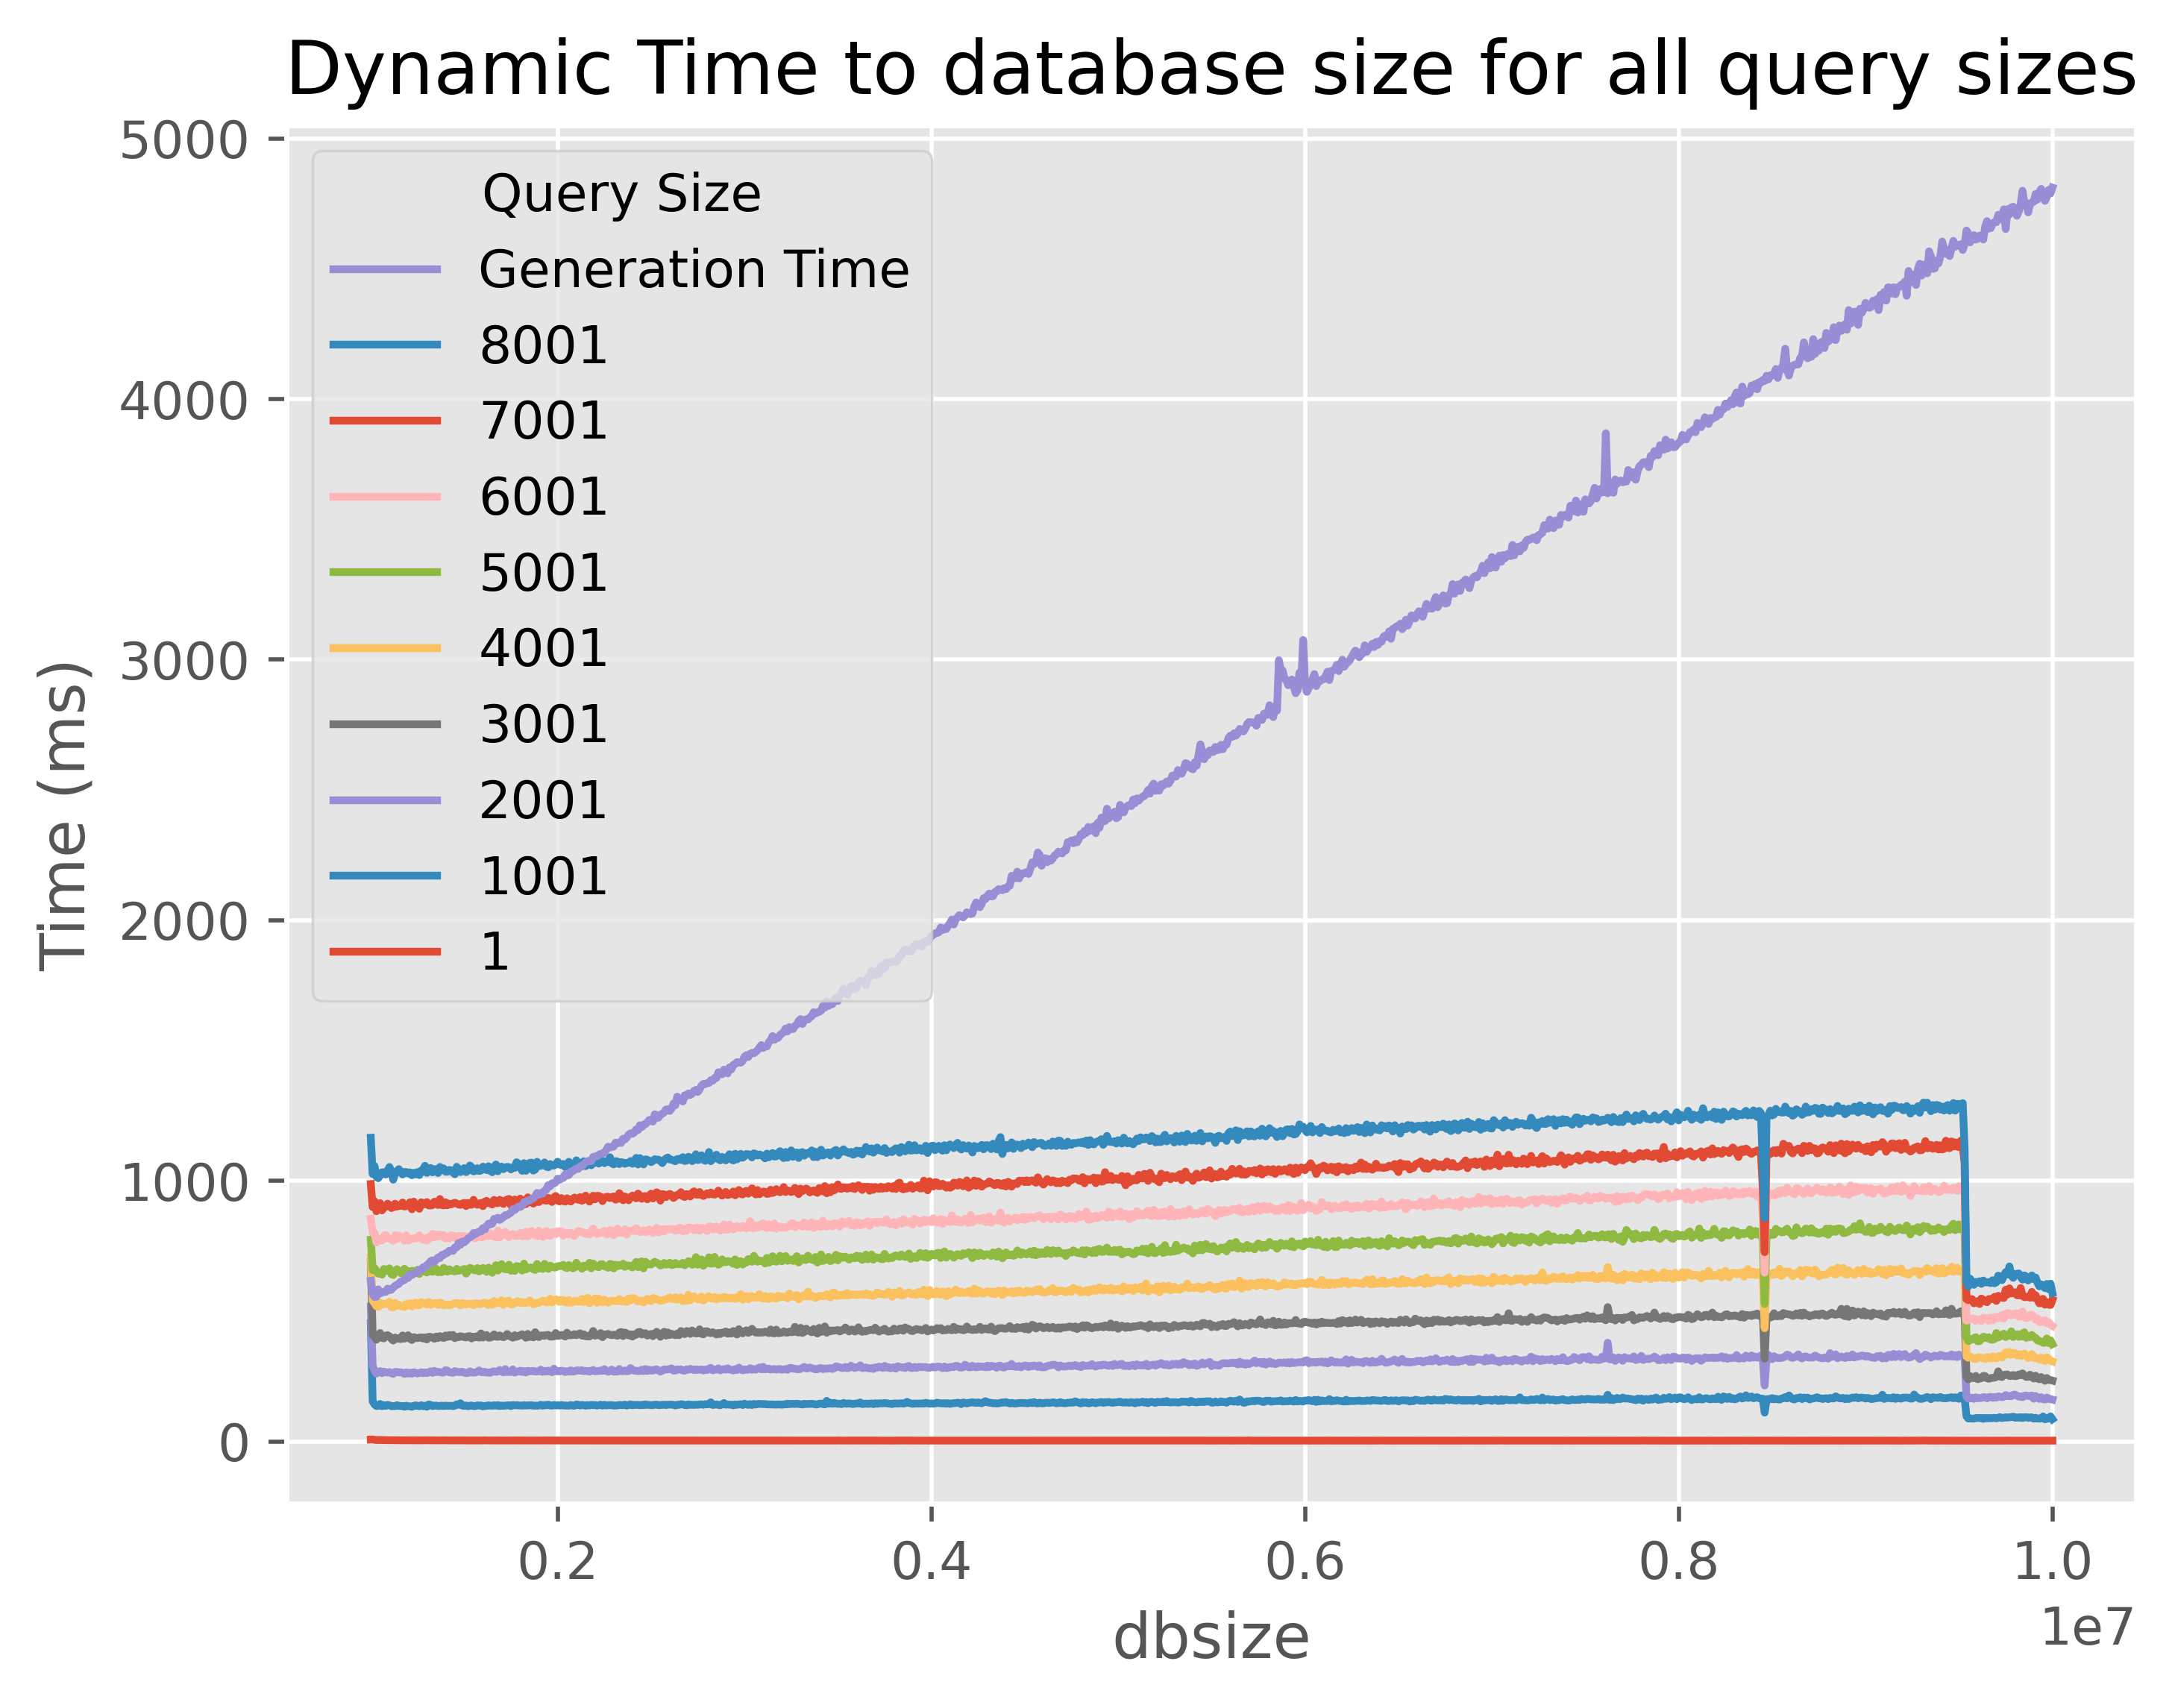
\includegraphics[width=0.8\textwidth]{figures/comparison-Generation-vs-Update.png}
    \caption{Comparison between the time it takes to generate a VoID description and the time it takes to update a VoID description, based on database size.}
    \label{fig:comparison-generation-vs-update}
\end{figure*}

\subsection*{Accuracy of generated VOID descriptions}

The last experiment tests the dynamic and generation methods for generating accurate void descriptions for an RDF database. Ensuring that both methods effectively produce the same void descriptions is crucial, as this is a critical benchmark for their reliability and accuracy. The premise is that the generation method always creates the correct void description. By filling the database with inserts of size 10,000 triple, applying both methods and checking if they create the same void description, we can assess the ability to generate correct void descriptions. Verifying the consistency of the dynamic method is essential for establishing its effectiveness.


The experiment started by initializing the Void_description objects one for the dynamic method (dyn_void_description) and one for the generation method (gen_void_description). These objects were used for the storage and comparison of the VoID descriptions of the RDF database, including the triple count, unique subjects count, unique predicates count, and unique objects count.

The code that does this can be seen here.
\begin{figure*}[t]
    \centering
    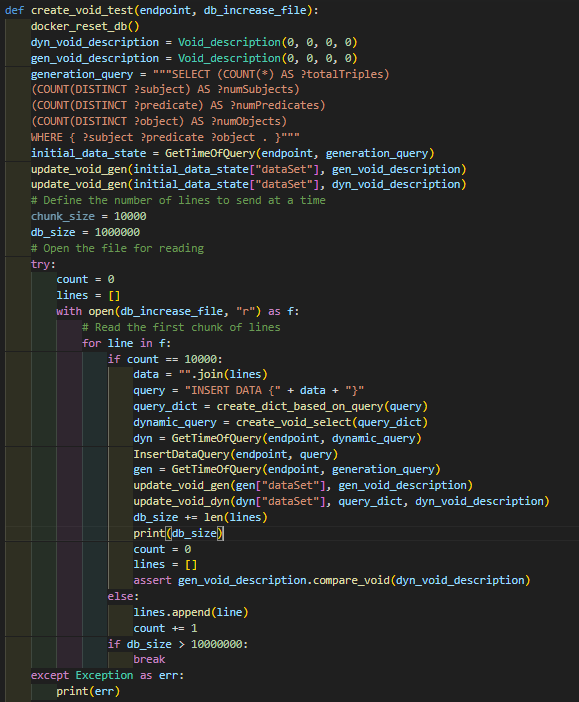
\includegraphics[width=0.8\textwidth]{figures/VOID-gen-test.png}
    \caption{Code snippet for VOID gen test}
    \label{fig:VOID-gen-test}
\end{figure*}

\begin{itemize}
    \item The initial state of the database was determined by executing a generation query (generation_query) using the GetTimeOfQuery function.
    
    \item The Void descriptions for both methods were updated based on the initial state using the update_void_gen function. This means their base values are set based on the initial state of the database.
    
    \item The experiment proceeded by reading the file containing the database inserts (db_increase_file) in chunks of 10,000 lines. For each chunk:
    
    \begin{itemize}
        \item The lines were processed to create an insert query.
        
        \item The insert query was executed using the InsertDataQuery function.
        
        \item The execution times and the response from the database for both the generation method query and the dynamic method query were measured using the GetTimeOfQuery function.
        
        \item The Void descriptions were updated accordingly using the update_void_gen and update_void_dyn functions.
        
        \item The database size was tracked by incrementing it based on the number of lines processed.
        
        \item The Void descriptions generated by both methods were compared using the compare_void method of the Void_description class to ensure consistency.
        
        \item If the database size exceeded a threshold of 10,000,000, the experiment was terminated.
    \end{itemize}
    
    \item If the script concludes, the voids must have been identical due to the assert used.
\end{itemize}



The experiment was successfully conducted, and the script ran to completion, demonstrating the functionality of both the generation and dynamic methods in creating statistics for the RDF database. The experiment aimed to compare the Void descriptions generated by these methods and ensure their consistency.
During the execution of the script, the database inserts were processed in chunks of 10,000 lines. As the experiment progressed, the database size increased, eventually reaching 10000000. At this point, both the generation method and the dynamic method had generated Void descriptions that captured the statistics of the RDF database.
To illustrate the Void descriptions generated by both methods at the database size of 8,500,000 triples, Figure X shows a comparison of these descriptions. The figure provides insights into whether the descriptions are identical at a given point; here, we see they are identical.
\begin{listing}[!ht]
    \begin{minted}[frame=single]{sparql}
        prefix rdf: <http://www.w3.org/1999/02/22-rdf-syntax-ns#>
        prefix rdfs: <http://www.w3.org/2000/01/rdf-schema#>
        prefix void: <http://rdfs.org/ns/void#>
        
        <test.com> a void:Dataset ;
            rdfs:label "dyn_void_description" ;
            void:uriSpace "test.com" ;
            void:triples 8566226 ;
            void:entities 1000965 ;
            void:properties 46 ;
            void:distinctSubjects 354526 ;
            void:distinctObjects 646393 .
        
        prefix rdf: <http://www.w3.org/1999/02/22-rdf-syntax-ns#>
        prefix rdfs: <http://www.w3.org/2000/01/rdf-schema#>
        prefix void: <http://rdfs.org/ns/void#>
        
        <test2.com> a void:Dataset ;
            rdfs:label "gen_void_description" ;
            void:uriSpace "test2.com" ;
            void:triples 8566232 ;
            void:entities 1000971 ;
            void:properties 46 ;
            void:distinctSubjects 354529 ;
            void:distinctObjects 646396 .
    \end{minted}
\end{listing}
Overall, the experiment yielded successful results, with the script running to completion and showcasing the effectiveness of both the generation and dynamic methods in creating statistics for the RDF database. 










% \begin{figure}[htb!]
%     \centering
%     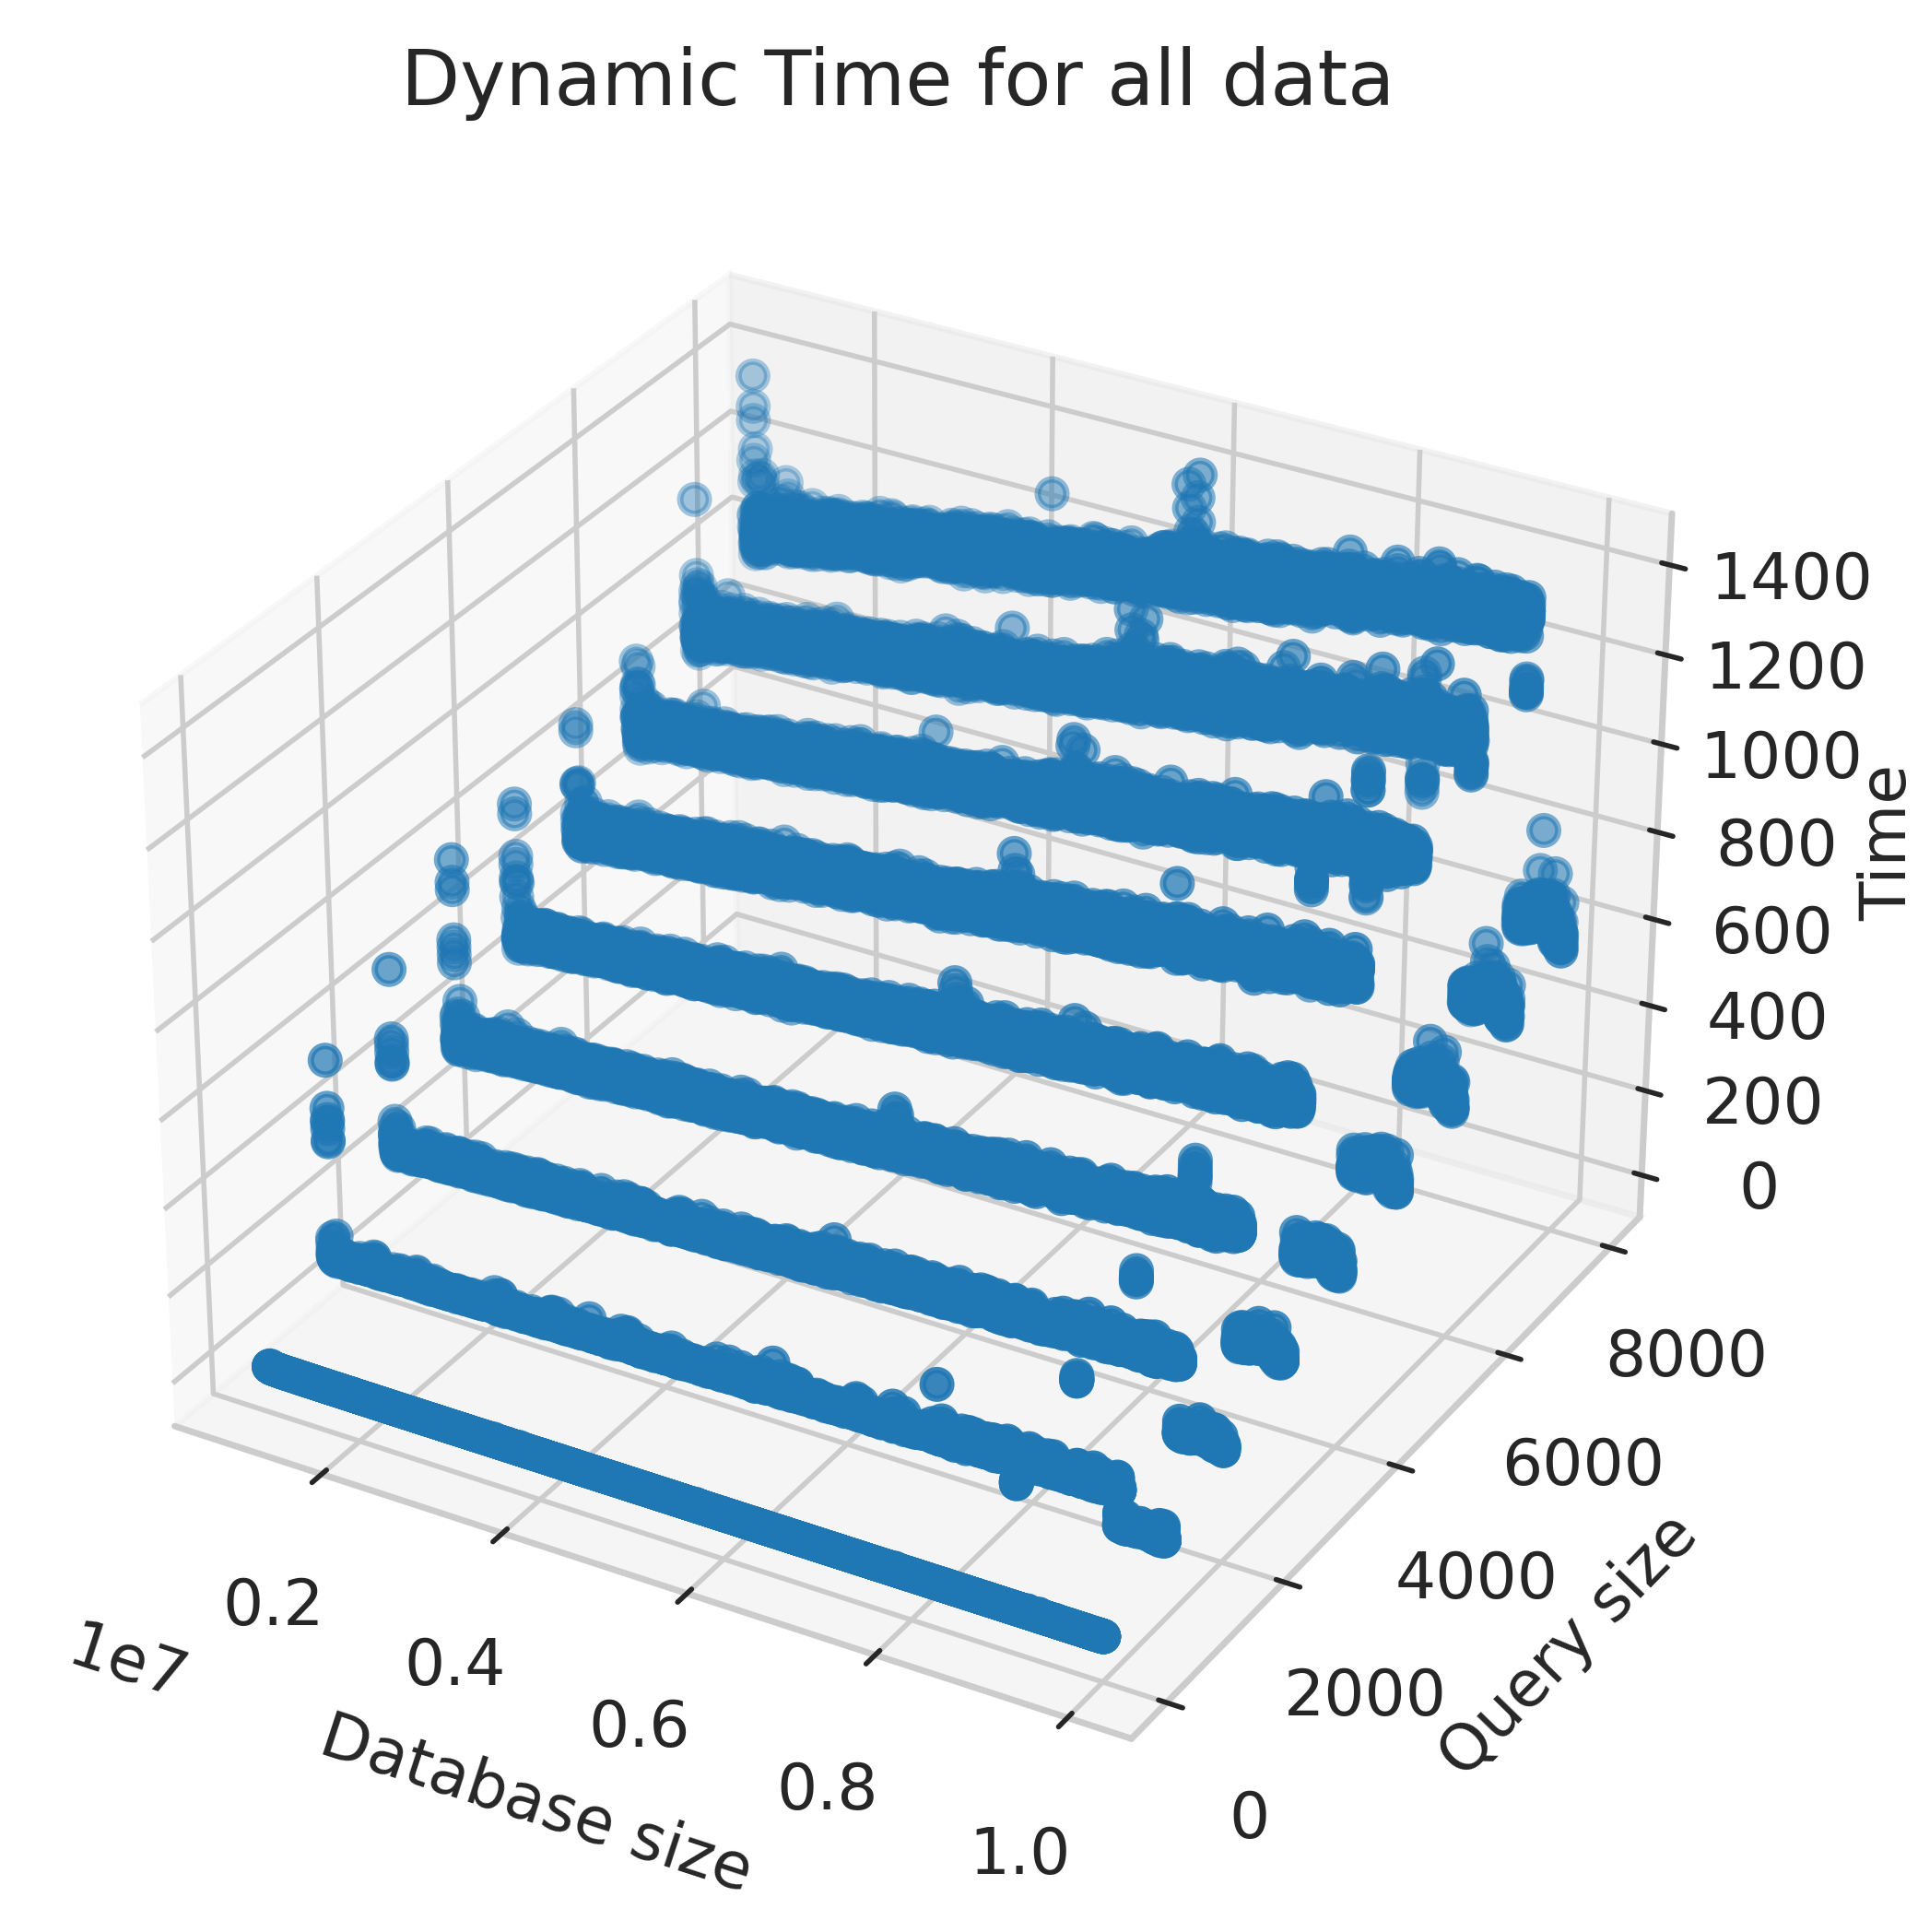
\includegraphics[width=0.8\columnwidth]{figures/dynamic-time-for-all-good.png}
%     \caption{3D graph showing the impact of query size and database size on the time it takes to update a VoID description, containing only the good data.}
%     \label{fig:update-querysize-dbsize-good}
% \end{figure}

% \begin{figure}[htb!]
%     \centering
%     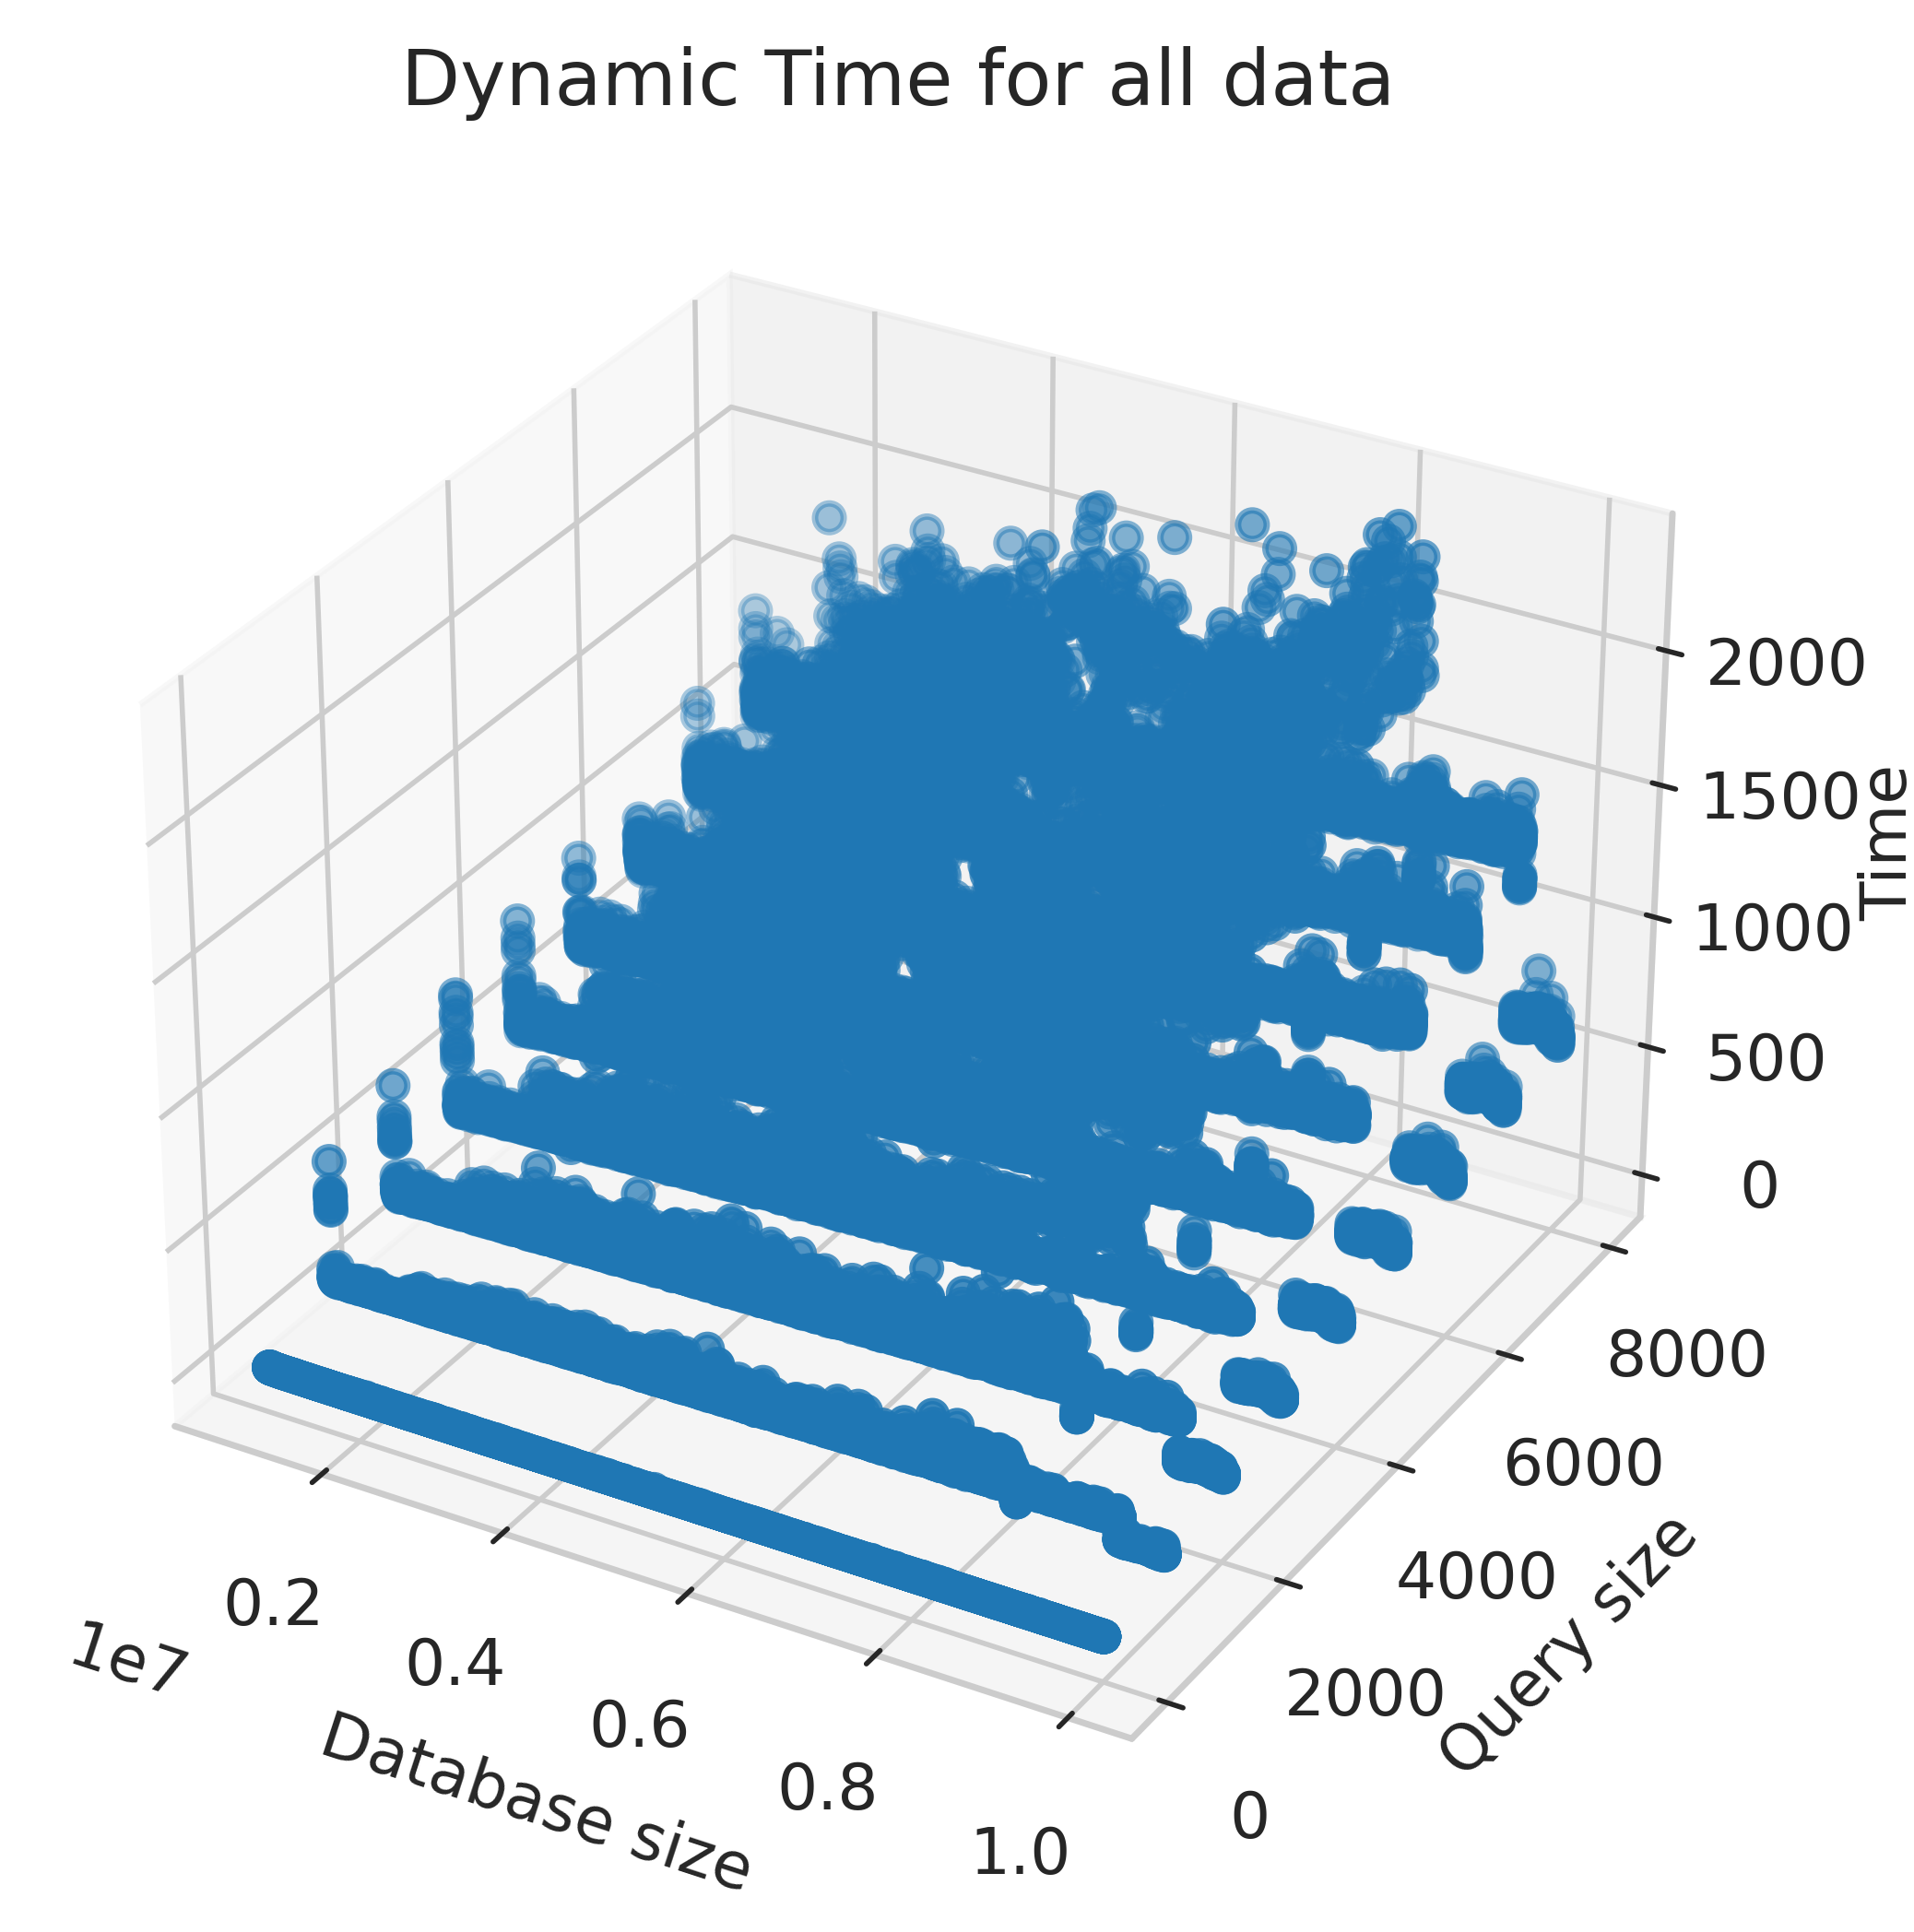
\includegraphics[width=0.8\columnwidth]{figures/dynamic-time-for-all.png}
%     \caption{3D graph showing the impact of query size and database size on the time it takes to update a VoID description, containing all the data.}
%     \label{fig:update-querysize-dbsize-all}
% \end{figure}

% \begin{figure}
%     \centering
%     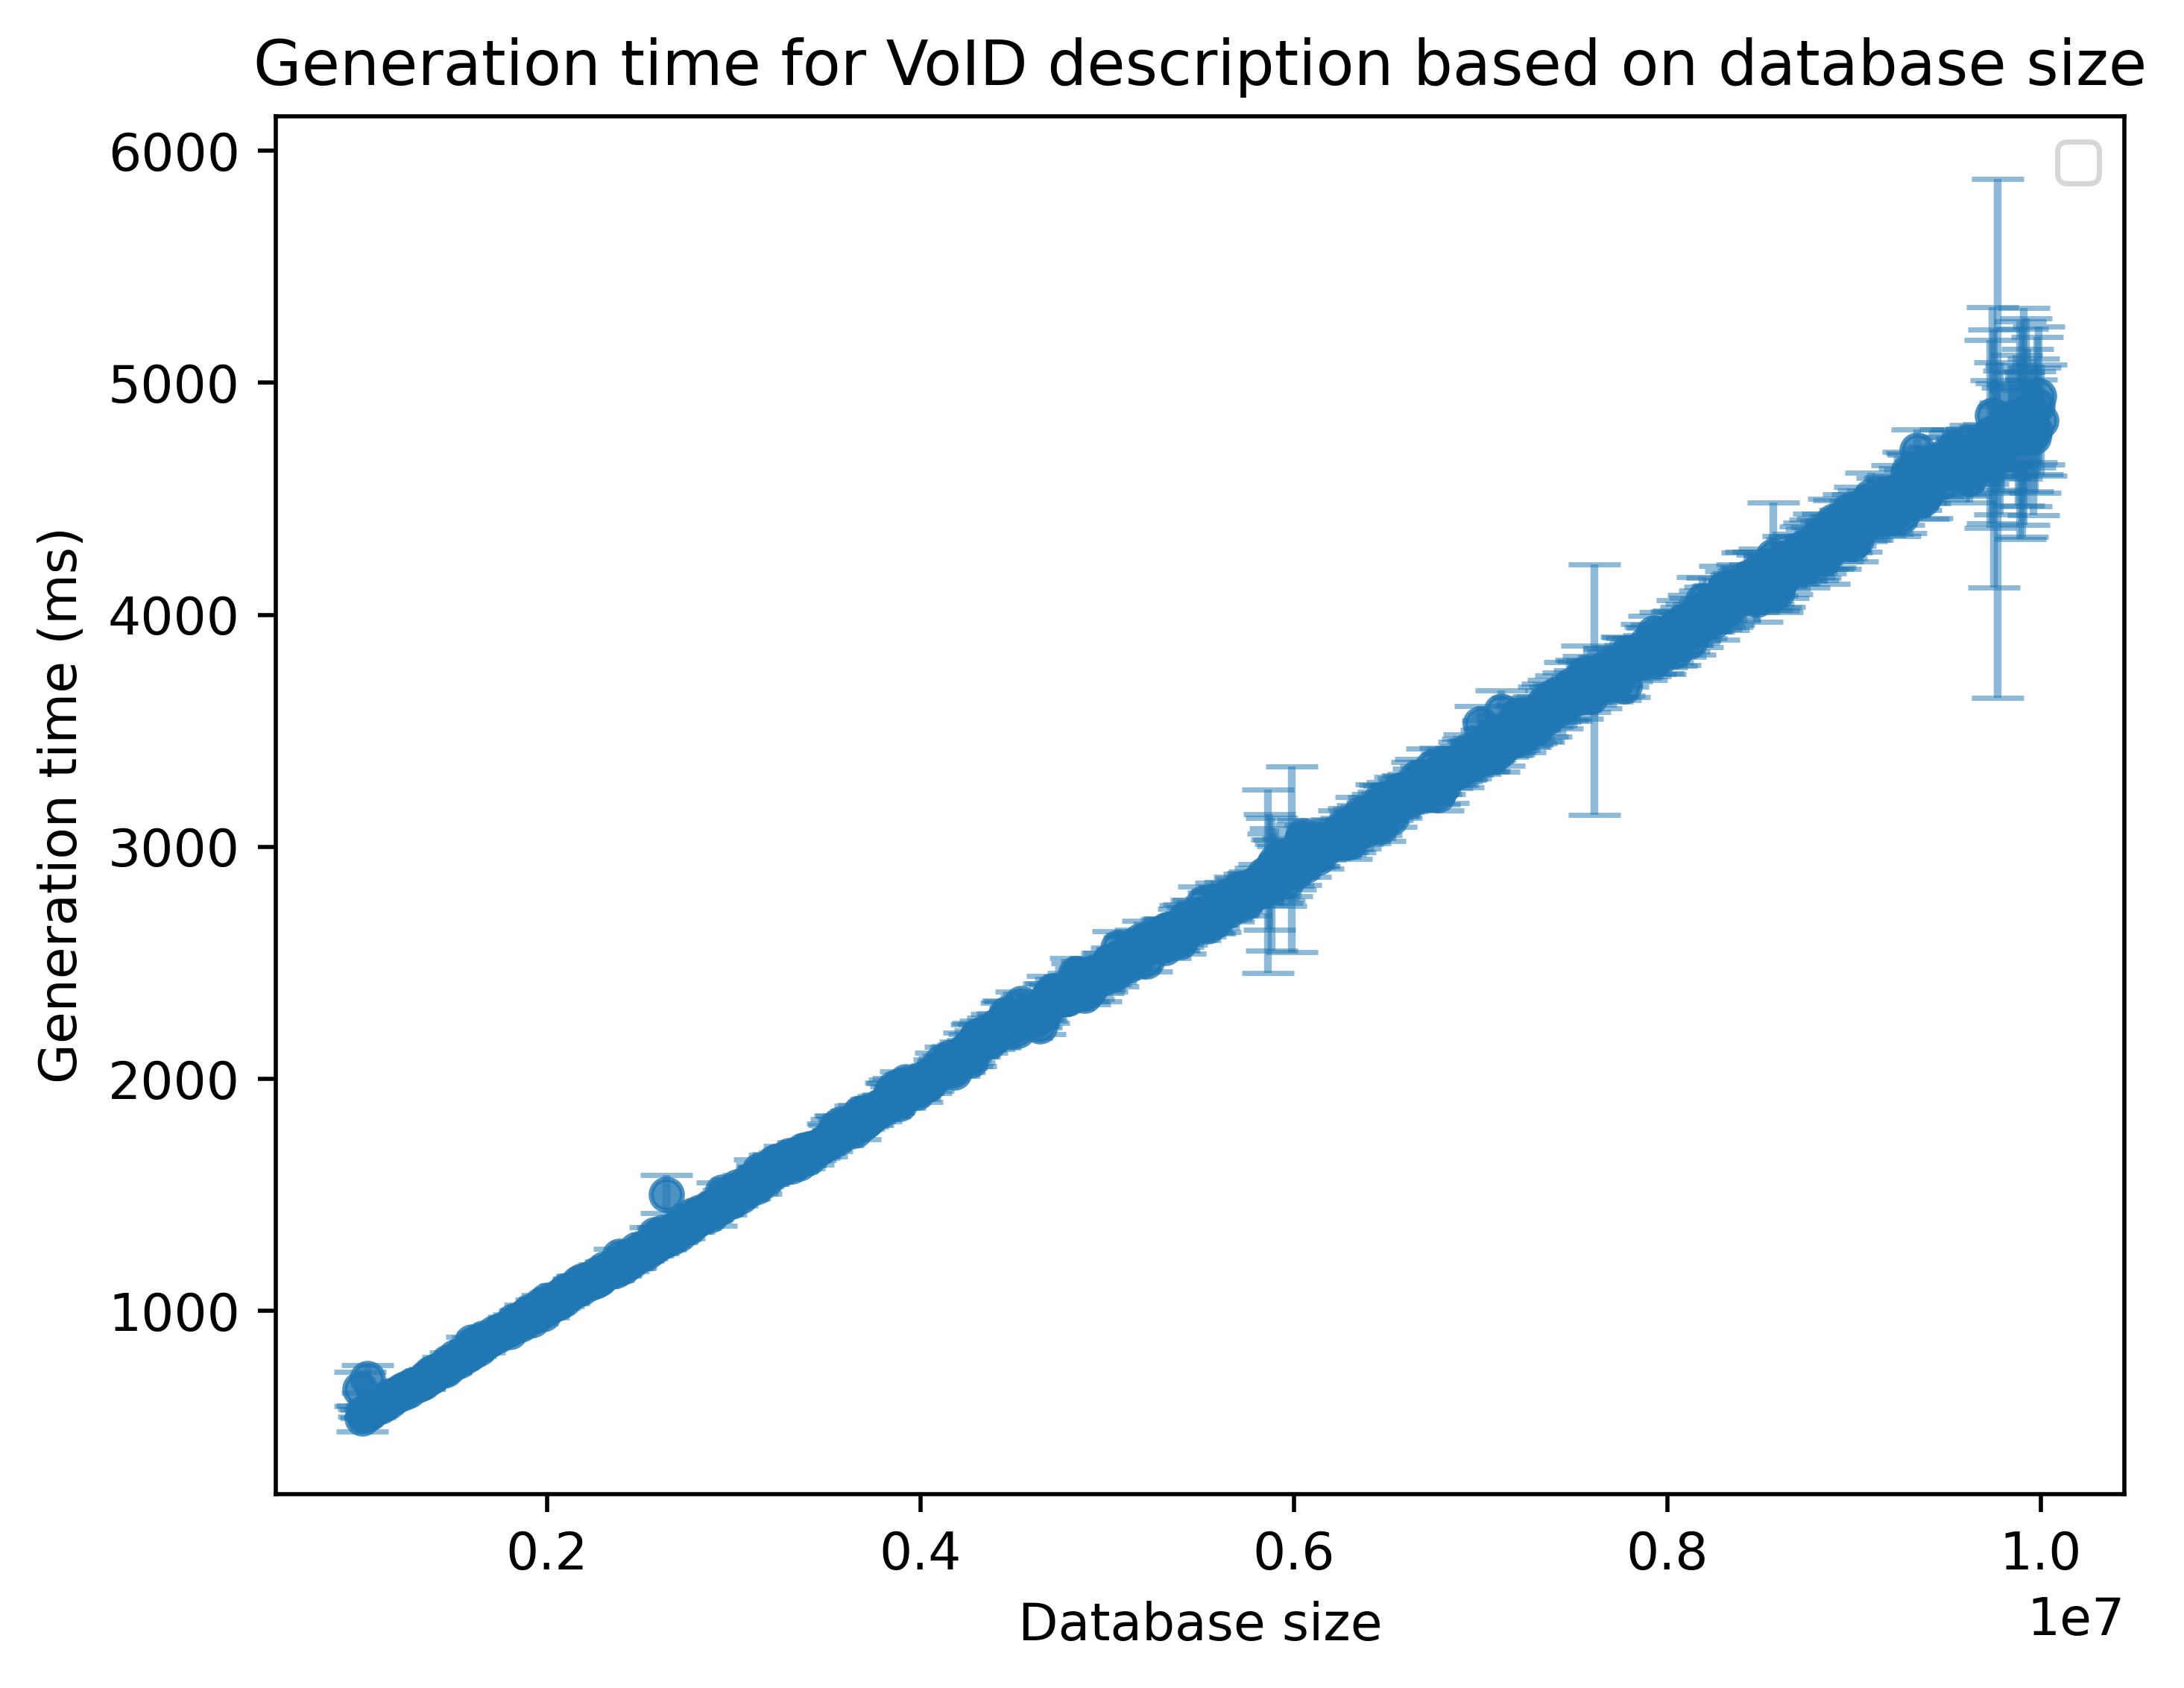
\includegraphics[width=0.8\columnwidth]{figures/generation-results-graph-good.png}
%     \caption{2D graph showing the standard deriviation impact of database size on the time it takes to generate a VoID description. Containing only the good data.}
%     \label{fig:generate-dbsize-good}
% \end{figure}



